\documentclass[10pt,a4paper]{article}
\usepackage[margin=1.35cm]{geometry}
\usepackage[T1]{fontenc}
\usepackage[utf8]{inputenc}
\usepackage{lmodern}
\usepackage{microtype}
\usepackage{booktabs}
\usepackage{array}
\usepackage{graphicx}
\usepackage[table]{xcolor}
\usepackage{hyperref}
\usepackage{fancyhdr}
\usepackage{tabularx}
\usepackage{amsmath}

\setlength{\parindent}{0pt}
\setlength{\parskip}{2.5pt}
\renewcommand{\arraystretch}{1.08}
\pagestyle{fancy}
\fancyhf{}
\lhead{CSC2042S Assignment 2}
\rhead{Sanele Hopewell Nkosi}
\cfoot{\thepage}
\hypersetup{colorlinks=true,linkcolor=black,urlcolor=blue}

\begin{document}

\begin{center}
{\Large\bfseries Multinomial Logistic Regression for Multilingual News Classification}\\[2pt]
{\large CSC2042S Assignment 2}\\[4pt]
\textbf{Name:} Sanele Hopewell Nkosi \hfill
\textbf{Student number:} nkssan033
\end{center}
\vspace{-5pt}\hrule\vspace{4pt}

\section{Object-oriented design, preprocessing, and training}

\textbf{Object-oriented design.}
The classifier was implemented as a PyTorch class, \texttt{MultinomialLogisticRegression}, derived from \texttt{nn.Module}. Its single \texttt{nn.Linear} layer maps a document feature vector to one logit per news category. The \texttt{forward} method returns raw logits for cross-entropy loss, \texttt{compute\_probabilities} applies softmax across the class dimension, and \texttt{predict} returns the class with maximum probability. The remaining pipeline was divided into functions for reading and cleaning data, encoding labels, generating mini-batches, creating feature representations, training configurations, evaluating models, sampling, bilingual training, and metric calculation. The \texttt{select\_best\_tuning\_result} function compares BoW, Binary, and TF--IDF results for one language using development accuracy, with lower development loss as a tie-breaker. This separation reduces repeated code and keeps model selection independent of test performance.

\textbf{Data processing.}
For English, isiXhosa, and chiShona, the headline and article body were combined. Text was converted to lowercase, punctuation was removed, and repeated whitespace was collapsed. Lowercasing avoids treating capitalisation variants as different features, while punctuation removal reduces sparse, low-information vocabulary entries. Tokenisation was performed by the default scikit-learn vectoriser analyser. Stop-word removal, stemming, and lemmatisation were not used because language-specific resources and morphological rules differ across the three languages. Avoiding English-specific rules reduced the risk of incorrectly altering informative isiXhosa and chiShona forms, although it increased vocabulary size and retained singular/plural variants.

\textbf{Training setup.}
Models were trained with shuffled mini-batches, stochastic gradient descent, and multiclass cross-entropy loss. Raw logits were passed directly to cross-entropy because PyTorch performs the required log-softmax internally. For every batch, gradients were reset, loss was backpropagated, and the optimiser updated the parameters. Sparse matrices were converted to dense tensors per batch. Tuning used a maximum of 50 epochs and early stopping with patience five, based on development loss. This limited unnecessary training and overfitting while retaining the model state from the best development-loss epoch.

\section{Feature extraction and hyperparameter tuning}

BoW records token counts, Binary records only presence or absence, and TF--IDF downweights tokens that occur in many documents. Vectorisers were fitted only on training text and then used to transform development and test text. A separate grid search was run for each language--representation pair over learning rates $\{0.1,0.5,1.0\}$, batch sizes $\{64,128,256\}$, maximum vocabulary sizes $\{5000,10000,20000\}$, and \texttt{min\_df} values $\{0,3,5,10\}$. Since scikit-learn does not accept integer \texttt{min\_df}=0, zero was implemented as 1, meaning no additional rare-term filtering. Selection was based only on development data.

\begin{table}[htbp]
\centering
\small
\caption{Best development and test accuracy for every language--feature combination.}
\begin{tabular}{llrr}
\toprule
Language & Representation & Dev. (\%) & Test (\%)\\
\midrule
English & BoW & 88.56 & 89.03\\
English & Binary & \textbf{88.77} & 89.77\\
English & TF--IDF & 87.92 & 90.30\\
\midrule
isiXhosa & BoW & 91.84 & 90.57\\
isiXhosa & Binary & \textbf{93.20} & 89.56\\
isiXhosa & TF--IDF & 88.44 & 86.53\\
\midrule
chiShona & BoW & \textbf{90.27} & 90.24\\
chiShona & Binary & 88.65 & 91.06\\
chiShona & TF--IDF & \textbf{90.27} & 92.95\\
\bottomrule
\end{tabular}
\end{table}

\begin{table}[htbp]
\centering
\small
\caption{Overall development-selected configuration for each language.}
\begin{tabular}{llrrrrr}
\toprule
Language & Feature & LR & Batch & Max vocab. & min\_df & Epoch\\
\midrule
English & Binary & 1.0 & 128 & 10000 & 10 & 11\\
isiXhosa & Binary & 1.0 & 128 & 10000 & 5 & 38\\
chiShona & TF--IDF & 1.0 & 64 & 5000 & 10 & 50\\
\bottomrule
\end{tabular}
\end{table}

Learning rate strongly affected how quickly configurations converged within the 50-epoch limit, but its effect interacted with representation, batch size, vocabulary size, and \texttt{min\_df}. The final selected English and isiXhosa configurations both used learning rate 1.0 and batch size 128. Smaller batches produced more parameter updates per epoch, while larger batches reduced update noise but sometimes converged less effectively. Increasing vocabulary size improved coverage but increased computation and could retain rare, dataset-specific words. Higher \texttt{min\_df} reduced dimensionality and noise, although aggressive filtering could remove useful topic words in the smaller African-language datasets.

Binary features achieved the highest development accuracy for English and isiXhosa, indicating that word presence was often more informative than repeated frequency. For chiShona, BoW and TF--IDF tied at 90.27\%; lower development loss selected TF--IDF. Test results were not used to revise these decisions. For example, English TF--IDF obtained 90.30\% on the test set, but Binary remained the correct development-selected English model.

\begin{figure}[htbp]
\centering
\IfFileExists{validation_loss_curve.png}{
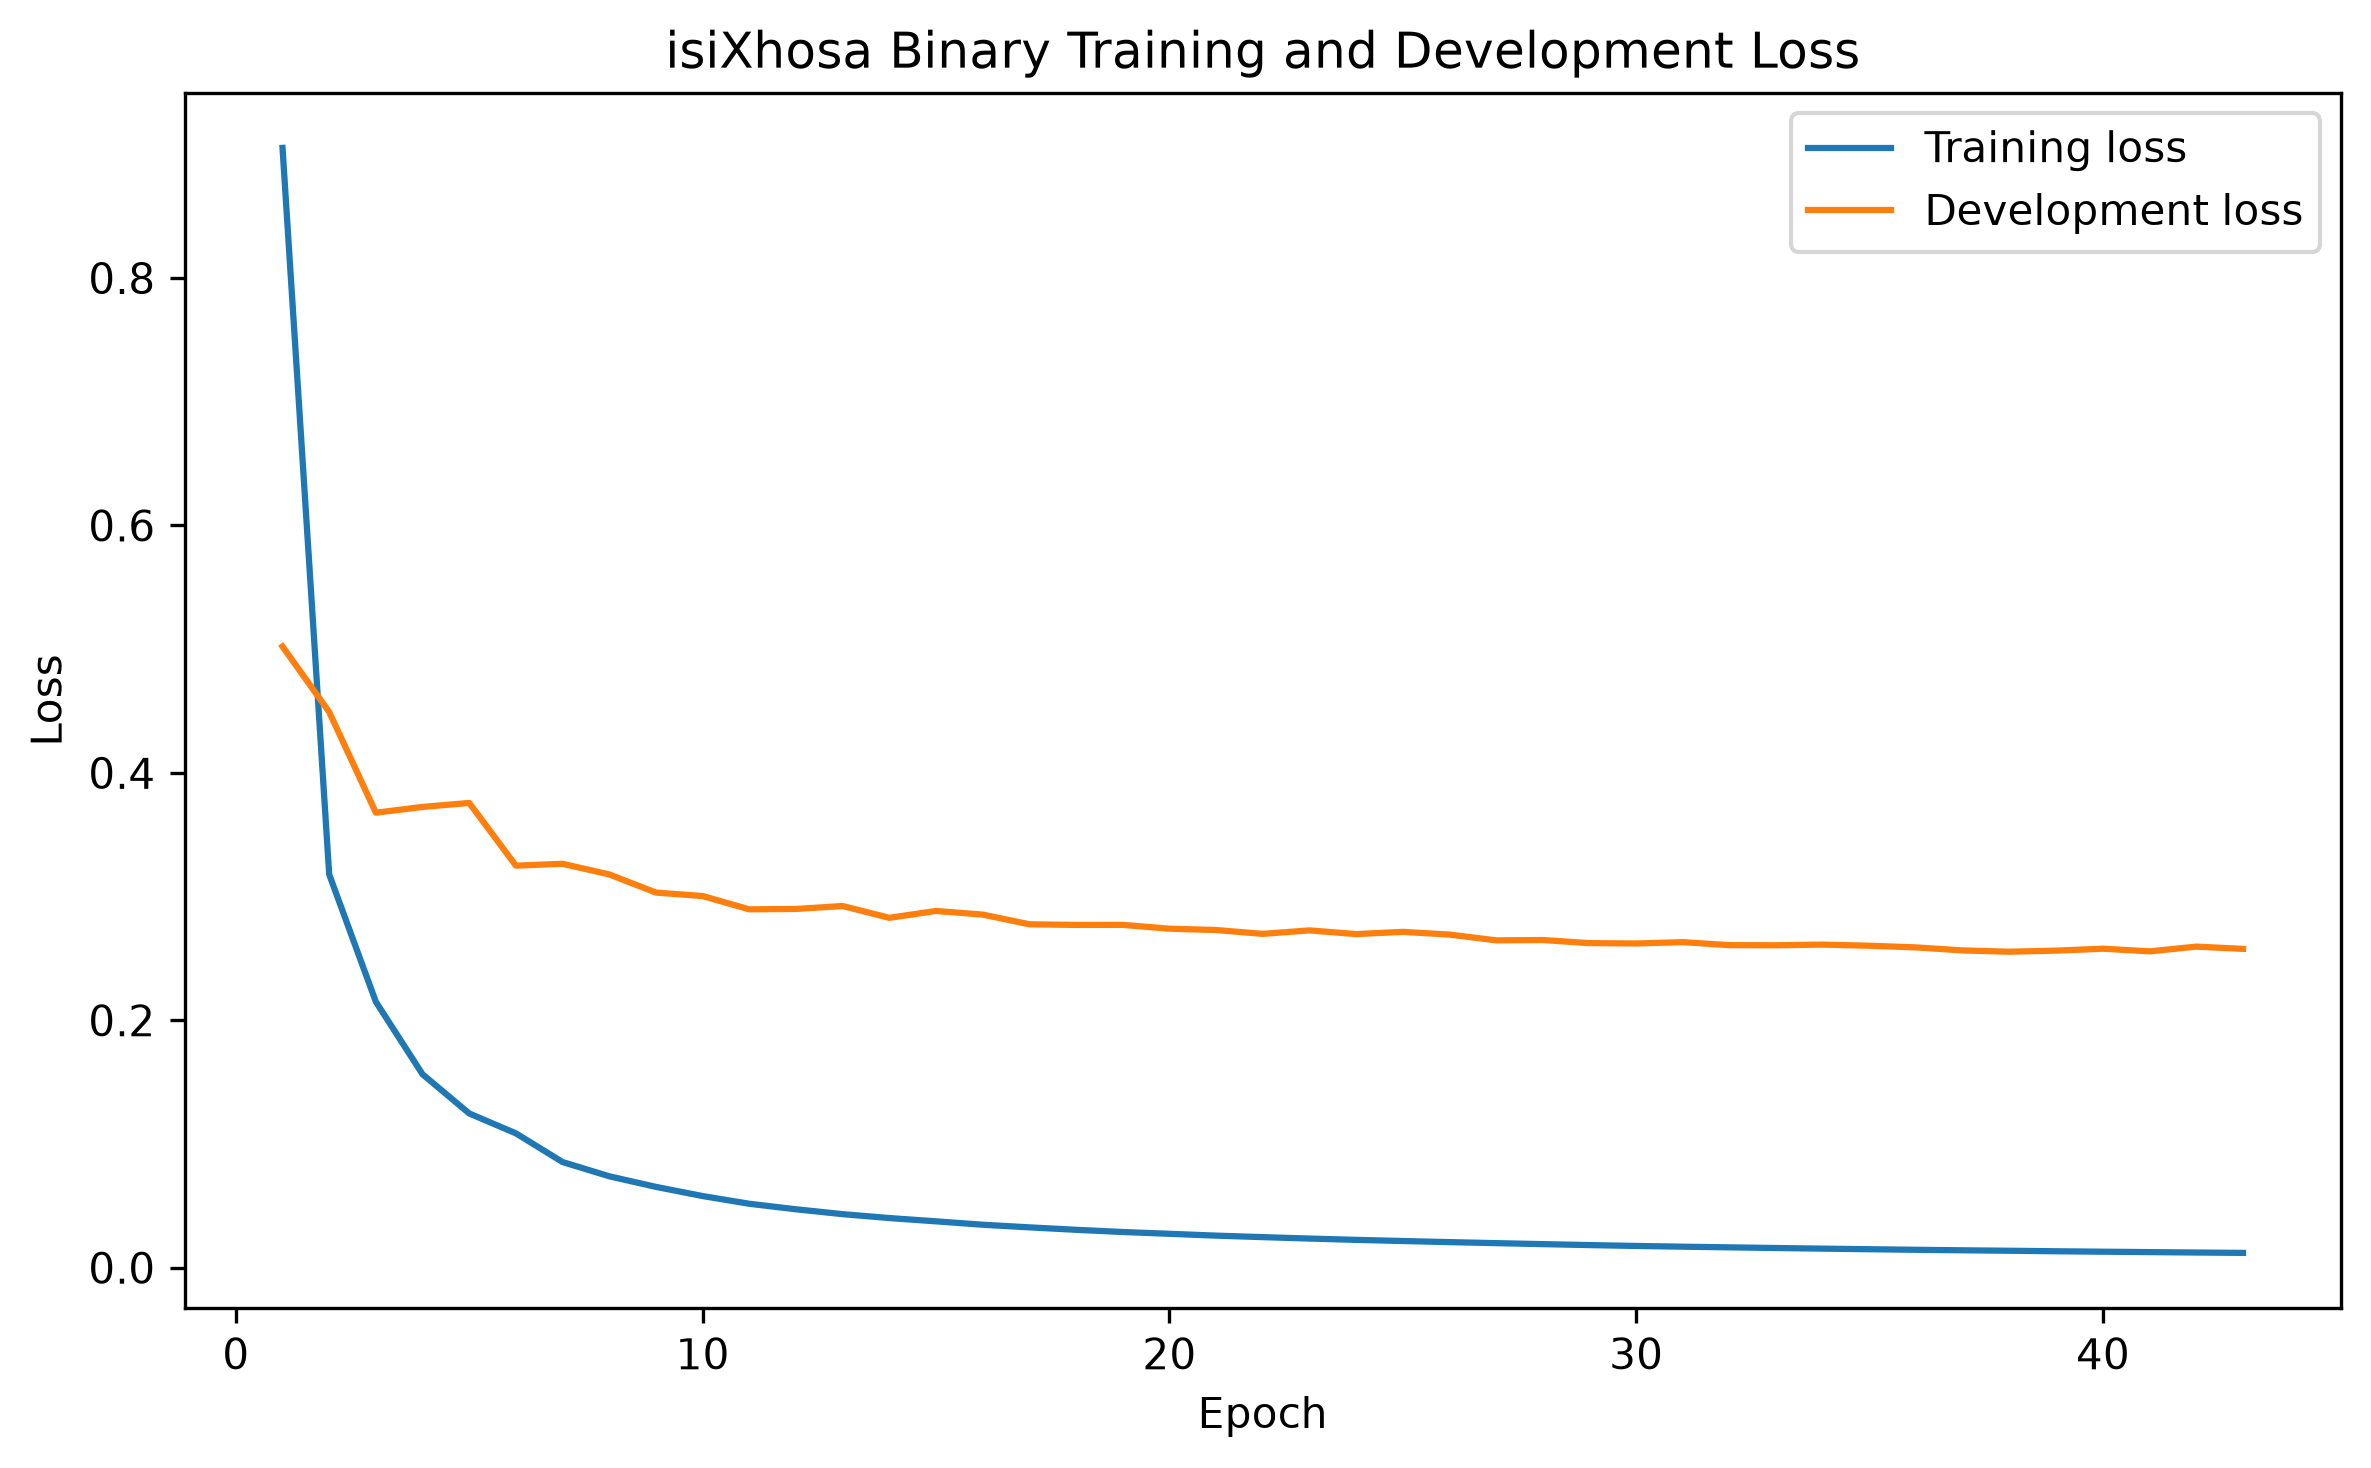
\includegraphics[width=0.61\linewidth]{validation_loss_curve.png}
}{
\fbox{\parbox[c][3.2cm][c]{0.58\linewidth}{\centering Export the selected model's notebook loss plot as\\\texttt{validation\_loss\_curve.png}.}}
}
\caption{Training and development loss for a development-selected configuration.}
\end{figure}

\section{Weight analysis}

English was selected because its learned associations could be interpreted directly. Its selected Binary model used 8,675 features. Large positive weights represented words whose presence raised a category logit. Business was associated with \emph{business}, \emph{company}, \emph{customers}, \emph{firm}, and \emph{bank}; entertainment with \emph{music}, \emph{show}, \emph{art}, \emph{artist}, and \emph{singer}; health with \emph{health}, \emph{NHS}, \emph{hospital}, \emph{patients}, \emph{COVID}, and \emph{cancer}; and sport with \emph{sport}, \emph{games}, \emph{Olympic}, and \emph{athletes}. These are plausible topic associations. The politics class also assigned high weights to \emph{Rishi}, \emph{Sunak}, and \emph{Welsh}, while technology included \emph{Elon}. These proper names can be useful in this dataset, but may encode particular news cycles rather than stable topic meaning, so they are plausible examples of dataset-specific overfitting. Separate weights for \emph{company}/\emph{companies} and \emph{artist}/\emph{artists} also show the effect of not applying lemmatisation.

\section{isiXhosa class imbalance}

The isiXhosa training counts were business 50, entertainment 350, health 70, politics 215, and sports 347. The best Task 5 isiXhosa representation and hyperparameters were retained while sampling rate changed. Upsampling used inverse-frequency weights with replacement so minority examples were repeated more often. Downsampling used lower majority-class weights without replacement and gradually moved the sample size towards a balanced dataset.

\begin{table}[htbp]
\centering
\small
\caption{isiXhosa development accuracy across sampling rates.}
\begin{tabular}{lrrr}
\toprule
Strategy & 0.50 & 0.75 & 1.00\\
\midrule
Upsampling & 92.52 & 92.52 & \textbf{93.20}\\
Downsampling & 87.76 & \textbf{91.84} & 91.84\\
\bottomrule
\end{tabular}
\end{table}

The best upsampling rate was 1.00. The best downsampling rate was 0.75, selected as the first rate reaching the tied maximum development accuracy. Test accuracy was 89.56\% without sampling, 90.24\% with upsampling, and 89.90\% with downsampling. Both strategies improved slightly over the baseline, but upsampling gave the larger gain of 0.68 percentage points and also improved macro recall from 0.7511 to 0.7938.

\section{Bilingual training}

Before observing results, isiXhosa+chiShona was expected to help isiXhosa more than isiXhosa+English because isiXhosa and chiShona were expected to share more relevant lexical structure. Each pair used one shared category mapping and one shared vectoriser fitted on combined training text. The isiXhosa-selected Binary representation, learning rate, batch size, and \texttt{min\_df} were retained, while vocabulary sizes 5,000, 10,000, and 20,000 were compared.

\begin{table}[htbp]
\centering
\small
\caption{Bilingual development and test results.}
\begin{tabular}{lrrrr}
\toprule
Pair & Best vocab. & xho dev. & Other dev. & xho test\\
\midrule
isiXhosa + chiShona & 20000 & 91.16 & 87.03 & 89.56\\
isiXhosa + English & 20000 & \textbf{92.52} & 87.92 & \textbf{90.24}\\
\bottomrule
\end{tabular}
\end{table}

At vocabulary sizes 5,000, 10,000, and 20,000, isiXhosa development accuracy for the chiShona pair was 89.12\%, 90.48\%, and 91.16\%; for the English pair it was 89.12\%, 89.80\%, and 92.52\%. Both therefore selected 20,000. In the selected isiXhosa+chiShona vocabulary, 6,545 terms occurred in isiXhosa and 6,876 in chiShona. In the isiXhosa+English vocabulary, 7,723 terms occurred in isiXhosa and 13,848 in English, showing stronger English dominance. Contrary to the prediction, isiXhosa+chiShona merely matched the 89.56\% monolingual baseline, whereas isiXhosa+English reached 90.24\%. Joint training with English therefore helped overall accuracy slightly, despite English contributing considerably more vocabulary terms.

\section{Evaluation and combined isiXhosa comparison}

\begin{table}[htbp]
\centering
\scriptsize
\caption{Complete isiXhosa test-set evaluation.}
\begin{tabular}{lrrrrrrr}
\toprule
Model & Acc. & Mic P & Mic R & Mic F1 & Mac P & Mac R & Mac F1\\
\midrule
Monolingual Binary & .8956 & .8956 & .8956 & .8956 & .8993 & .7511 & .7895\\
\rowcolor{green!12}Upsampling & \textbf{.9024} & .9024 & .9024 & .9024 & .8989 & \textbf{.7938} & \textbf{.8282}\\
Downsampling & .8990 & .8990 & .8990 & .8990 & .8903 & .7531 & .7889\\
isiXhosa + chiShona & .8956 & .8956 & .8956 & .8956 & .8959 & .7431 & .7813\\
isiXhosa + English & \textbf{.9024} & .9024 & .9024 & .9024 & \textbf{.9032} & .7563 & .7940\\
\bottomrule
\end{tabular}
\end{table}

For the development-selected monolingual models, English Binary achieved accuracy/micro-F1 0.8977 and macro-F1 0.8944; isiXhosa Binary achieved 0.8956 and 0.7895; and chiShona TF--IDF achieved 0.9295 and 0.9305. In single-label multiclass classification, micro precision, recall, and F1 equal accuracy because decisions are pooled across all observations. Macro metrics weight each category equally. The much lower isiXhosa macro recall and macro F1 therefore show that strong majority-class performance hides weaker results for business and health.

\begin{figure}[htbp]
\centering
\IfFileExists{xhosa_confusion_matrix.png}{
\includegraphics[width=0.52\linewidth]{xhosa_confusion_matrix.png}
}{
\begin{tabular}{l|rrrrr}
 & Bus. & Ent. & Health & Pol. & Sport\\\hline
Business & \cellcolor{green!30}8 & 1 & 0 & 6 & 0\\
Entertainment & 0 & \cellcolor{green!45}93 & 0 & 4 & 3\\
Health & 0 & 5 & \cellcolor{green!35}12 & 3 & 0\\
Politics & 0 & 2 & 0 & \cellcolor{green!45}58 & 2\\
Sports & 0 & 1 & 0 & 2 & \cellcolor{green!45}97
\end{tabular}
}
\caption{Confusion matrix for the selected isiXhosa upsampling model.}
\end{figure}

The upsampling model classified entertainment, politics, and sports most reliably, with 93/100, 58/62, and 97/100 correct predictions. Business and health remained harder, with 8/15 and 12/20 correct. Business was mainly confused with politics, while health was confused with entertainment and politics. Upsampling produced the strongest rare-class result because macro recall rose to 0.7938 and macro F1 to 0.8282. Downsampling slightly increased accuracy but macro F1 fell to 0.7889. The English bilingual model tied upsampling on accuracy, but its lower macro recall of 0.7563 and macro F1 of 0.7940 show that the gain was concentrated more heavily in common classes. Thus, Task 7 upsampling was the best overall intervention when both aggregate and rare-class performance are considered.

\textbf{Conclusion.}
The linear classifier achieved strong multilingual news classification when representation and optimisation were selected separately by language. Binary features were selected for English and isiXhosa, while TF--IDF was selected for chiShona. Learning rate, batch size, vocabulary size, and frequency filtering interacted rather than having one universal optimum. Full upsampling gave the best balanced isiXhosa result. Bilingual English training matched the best accuracy but did less for rare classes, and the expected advantage of the more closely related chiShona pair was not observed.

\section*{AI Usage Statement} I used Claude and Microsoft 365 Copilot while completing this assignment. Claude was used to review the structure and completeness of the report, cross-check whether reported results were consistent with the outputs in my notebook, and identify sections that required further analysis or supporting evidence. Microsoft 365 Copilot was used to help interpret error messages, debug code, identify inconsistencies in the model-selection and evaluation pipeline, and improve the clarity, grammar, and organisation of my written explanations. I also used the Microsoft 365 to improve my LATEX code, by making it look more academically professional.

\end{document}
